\section{推理模型鲁棒性不足的可解释性分析}
%\section{常识性推理任务中的偏差识别与评估架构}



%在本章节的开篇,我们将聚焦人工智能领域的一个关键挑战:解析推理模型鲁棒性差的原因。
%如\secref{sec1:interpretability}所述,我们认识到,尽管利用如
%CheckList工具的现有评估方法为理解模型的鲁棒性提供了关键洞见,但这些方法在揭
%示模型确切学习内容及其背后的复杂动态方面显得力不从心。这突显出一个研究空白:目
%前对模型所学内容及其背后的复杂机制的理解,仍然缺乏系统性和深度。
%
%应对这一挑战,我们可以从两个角度出发:数据的角度或者模型的角度。因为最终应用的模型
%实体是数据和模型结构共同作用的结果。在本节的研究中,我们主要从\textbf{数据的角度}进行分析解释。

在\secref{sec1:interpretability}中,我们深入探讨了模型在处理常
识性推理任务时表现的鲁棒性不足的现象以及这个现象的可解释性上。
虽然这些模型在标准测试环境下展现出色,但它们在面对对抗性数据或
与训练环境截然不同的情形时,却展现出显著的脆弱性。众多研究提出了一个
关键假设,即这种鲁棒性不足可能源自模型对数据中特定结构元素的过度依赖,
如偏见线索或虚假线索。这一假设背后的深层次原因在于数据集的构建方式,
这导致模型倾向于学习数据特有的简化规则而非广泛适用的解决策略。

为了对这一假设进行验证,研究者们引入了``仅假设''测试和注意力图等工具。
这些方法使研究者能够更深入地分析模型可能对数据中某些特定结构元素的过分关注。
然而,这些方法在解释模型行为方面存在一定的局限性。例如,``仅假设''测试并不能
充分展现模型在处理真实场景时的推理模式,因为它的测试数据结构与模型在训练阶
段所接触的数据结构并不一致。同样,尽管注意力图被用来揭示模型的焦点,但相关
研究表明,模型通过注意力机制突出显示的内容并不总是准确反映其决策的真实依据。
鉴于此,深入探索
数据偏见如何具体作用于模型的机制已成为一个迫切且重要的研究课题。

我们将在本章介绍两种创新的测试框架,用以深入分析并理解数据偏见对模型鲁棒性的影响。
首先,我们提出的宏观层面测试框架,通过将测试数据划分为简单(easy)和困难(hard)两类,
对模型在识别和处理虚假特征方面的能力进行量化评估。此方法揭露了模型对特定统计规
律的过度依赖,帮助我们深入理解模型泛化能力的局限。

其次,我们引入了微观统计分析框架——ICQ(``I-see-cue'')框架,它通过多维特
征划分和细致的性能分析,探究模型在不同特征上的准确性和分布表现。此外,我们还
开发了一种直观的可视化工具,旨在更有效地识别和理解模型性能差异的根源。

总体而言,本研究的主要贡献在于这两种高度创新的分析框架,它们为深入解析常识性推理模型的鲁棒性不足问题
提供了新的路径。
%通过结合宏观与微观方法,我们能够全面
%评估模型在处理复杂数据时的行为模式,尤其是在识别和处理潜在虚假特征方面的能力。这些成
%果不仅揭示了模型的潜在薄弱环节,也为未来设计更加健壮且可解释的人工智能系统打下了坚实的基础。

\subsection{概述}
\label{sec4:intro}
深度神经网络模型在各种自然语言理解(NLU)任
务中取得了显著的成就,这些任务包括自然语言
推理~\cite{bowman2015large,wang2018glue}、论证分析~\cite{niven2019probing}、常
识推理~\cite{mostafazadeh2016corpus,roemmele2011choice,zellers2018swag}、阅读理
解~\cite{lai2017race}、问题回答~\cite{talmor2019commonsenseqa}和对话
分析~\cite{lowe2015ubuntu}。这些任务经常采用多项选择框架,正如在斯坦福
自然语言推理(SNLI)数据集的例子中所示(见 \exref{exp4:snli})。然而,近期研究~\cite{gururangan2018annotation,sanchez2018behavior,poliak2018hypothesis,checklist2020acl}揭示了
一些问题,特别是在这些模型对微小变化高度敏感的背景下,我们需要一个更为稳健且精确的评估机制。

\begin{center}
    \begin{example}\label{exp4:snli}
    SNLI 数据集中的自然语言推理示例,正确答案以斜体标出
    \begin{description}
    \item{Premise:} A swimmer playing in the surf watches a low flying airplane headed inland.
    \item{Hypothesis:} Someone is swimming in the sea.
    \item{Label:} \textit{a) Entailment.} b) Contradiction. c) Neutral.
    \end{description}
    \end{example}
    \end{center}
在处理类似 \exref{exp4:snli} 这样的任务时,人类通常依赖于前提和假设之
间的逻辑关系。与此相反,一些 NLP 模型可能会绕过这种逻辑推理,转而关注数据集
中嵌入的偏见,特别是在假设中的偏见~\cite{naik2018stress,schuster2019towards}。
这些偏见,如情感或表层 n-grams,可能为正确预测提供误导性线索。

当这些偏见在训练和测试数据集中普遍存在,并在预测上保持类似的分布时,我们将其
称为``人为虚假线索''(如图 \ref{fig4:cue_def} 所示)。例如,在 \exref{exp4:snli} 中,某
些模型可能过分依赖``someone''一词来做出判断。这种情况下,当这些线索缺失或改变时,可能会显
著影响模型的性能,凸显了识别这些线索以提高模型鲁棒性的重要性。

\begin{figure}[th]
\centering
\includegraphics[width=0.50\columnwidth]{figures/emnlp/cue_def.eps}
\caption{线索的示例。}
\label{fig4:cue_def}
\end{figure}


本研究旨在探讨如何在各类自然语言理解任务中识别和解决虚假线索的问题。
我们特别关注这些线索在数据集制作过程中如何产生,以及模型在训练过程
中如何学习并依赖这些线索。我们提出的方法旨在揭示这些线索,并帮助我们
深入理解它们如何影响模型的性能和推理能力。为此,我们将从宏观和微观两
个角度分析模型是否受到虚假线索的影响。

\subsubsection*{宏观角度分析}
我们提出了一种新方法,用以从宏观角度分析自然语言理解(NLU)任务中虚假线索的问题。
在探索人类处理这类问题的方式时,我们发现人们通常会仔细分析问题的前提和假设之间的
逻辑关系。然而,之前的研究~\cite{naik2018stress,schuster2019towards}显示,
许多自然语言处理(NLP)模型在处理类似问题时,往往只考虑假设部分,忽视了逻辑关系
的深入分析。这一现象在很大程度上归咎于数据集中人工制作的假设存在的瑕疵。

虽然``仅假设''测试在理论上是用于识别此类问题的有效方法,但它常依赖于特定
的、如BERT~\cite{devlin2018bert}这样的模型,这就需要进行模型的重新训练。
更重要的是,``仅假设''测试并不能
充分展现模型在处理真实场景时的推理模式,因为它的测试数据结构与模型在训练阶
段所接触的数据结构并不一致。

在我们的研究中,我们开发了一种轻量级框架,专注于识别多项选择自然语言
推理数据集中的关键且影响力显著的线索。尽管不是所有多项选择题都包含前
提、假设和标签,但我们在第 \ref{sec4:approach1} 节中详细介绍了如何将
这些元素标准化。我们的框架以词汇为基础,利用它们作为构建线索的关键特征,因
为词汇在大多数现代机器学习方法中是自然语言建模的基石。此外,即便是复杂的语
言特征,如情感、风格和观点,也通常是基于词汇特征。

我们的实验展示了,基于词汇的线索在检测数据集中的统计偏差方面,与资源消
耗更大的``仅假设''方法同样有效。这一发现对于理解和改进模型的推理能力至关重要。

此外,我们还设计了一种方法,将测试数据基于问题是否能仅通过线索特征被
正确回答的能力,划分为简单和困难两个子集。数据集中困难部分的相对大小是衡
量其整体质量的重要指标,其中困难部分占比越大,表明数据集质量越高。这种划分
同时也是一种``压力测试'',可用于评估模型的真实推理能力。两个子集间的分类准确
率差异揭示了模型在不同情境下的潜在薄弱环节。

%最后,我们还提出了一种划分训练数据的简单方法,将其分为简单和困难两部分。这样做的目的是,通过让模型专注于更复杂的线索,从而提高其在处理困难问题时的推理能力。

综上所述,这个宏观层面的方法的研究贡献有两个。首先,我们开发了一种轻量级但有效的方法,用
于评估和识别自然语言理解数据集中的统计偏见和虚假线
索(\secref{sec4:approach1}、\secref{sec4:experiment1} )。
另外,我们通过将测试数据划分为简单和困难两部分,根据信息泄露程度来
评估模型的真实推理能力,从而量化比较这两部分的性能差异(\secref{sec4:experiment1} )。

\subsubsection*{微观角度分析}
在微观层面上,我们的研究着重于区分数据集中预先嵌入的
线索与模型在训练过程中所学习的线索。传统的偏见检测与缓解工具,
如 AI Fairness 360 工具包~\cite{bellamy2018ai},尽管主要聚焦
于数据集中的偏见,但在处理模型训练过程中产生的偏见时,它们往往显示出局限性。

现有的方法,例如``仅假设''测试和 CheckList,虽然能够揭示模型的脆
弱性,却不是专门为识别模型学习的线索而设计的。具体来说,``仅假设''测试能
够突显出数据集中的某些问题,如仅凭假设就能得出正确答案的情况,但这并未涵盖
模型在训练和预测过程中使用的完整数据上下文,因此无法全面反映模型的整体能力。

同样地,虽然 CheckList 采用了软件工程中的黑盒测试原则,通过对预
定义语言特征的额外压力测试案例来审视模型的弱点,但它对精心设计的模板的
依赖限制了其应用范围。这种方法能够揭示模型的脆弱性,
%类似于我们在上一章
%节构造的代理测试(参见\secref{sec3:approach} 节),
但它并不能清楚地揭
示模型实际从数据中学到的具体知识或特征。

尽管我们的宏观架构能够在一定程度上分析模型受到数据中虚假线索的影响程度,
但它难以具体指出受到哪些特定线索的影响。

为了克服这些局限,我们引入了 ICQ(``I-see-cue'',意为``我发现线索''),
一个灵活的统计分析框架\footnote{代码和数据集可在 \url{https://github.com/flora336/icq} 获取}。
ICQ 的设计哲学与传统方法完全不同,它能够在不需要额外测试案例的情况下,有效识别多项选择
 NLU 数据集中的偏见。采用黑盒测试方法,ICQ 能够评估模型如何利用这些偏见,从而为理解
  NLU 任务中的偏见提供全面且深入的见解。

我们通过在不同的 NLU 数据集上部署 ICQ 来验证其有效性,并探索模型在训练
期间可能学习到的线索。ICQ 的应用极大地促进了我们对于诸如 ChatGPT%\footnote{\url{https://chat.openai.com/}}
这类模型如何学习潜在
线索的深入理解,并提供了选择合适提示的示例,为模型的优化提供了重要的指导。

综上所述,我们的微观研究主要提供了以下几点贡献:
\begin{itemize}
\item 我们推出了 ICQ,这是一种轻量级且功能强大的工具,专门用于识别 
NLU 数据集中的统计偏见和线索。我们还提出了简单而有效的测试方法,以量化和
直观地评估模型是否在其预测中利用了虚假线索。
\item 我们对十个流行的 NLU 数据集和四个模型进行了全面的统计偏见问题
评估,从而证实了先前的发现并揭示了新的见解。我们还提供了一个在线演示系
统,展示结果并邀请用户评估他们自己的数据集和模型。
\item 通过一个案例研究,我们深入探讨了 ChatGPT 如何学习潜在偏见,并为
其实际应用提供了宝贵的建议。
\end{itemize}

\subsection{相关工作}
\label{sec3:related}

我们的工作涉及三个研究方向:虚假特征分析、偏见计算和数据集过滤。

\subsubsection*{虚假特征分析}
近年来,虚假特征分析在自然语言处理(NLP)领域获得了越来越多的关注。研究表明,许多 NLP 模型能够在多项选择题形式的自然语言理解问题中取得良好表现,有时甚至无需深入理解问题的核心内容。这类现象在某些研究中被称为``仅假设''测试~\cite{sharma2018tackling,srinivasan2018simple,zellers2018swag}。此外,研究发现,这些模型对于假设中的微小但语义重大的变化并不敏感,推测这种``仅假设''表现可能源于假设中的词语与答案标签之间的简单统计关联~\cite{sanchez2018behavior}。

虚假特征可分为词汇化和非词汇化两类~\cite{bowman2015large}。词汇化特征主要包括 n-gram 词标和交叉 n-gram 词标,而非词汇化特征则涉及词汇重叠、句子长度以及前提和假设之间的 BLEU 分数。词汇化分类的细化,如否定、数值推理和拼写错误,也在文献中得到了探讨~\cite{naik2018stress}。另一方面,非词汇化特征如词汇重叠、子序列和成分被进一步细化,同时也考虑了句法结构重叠~\cite{mccoy2019right}。此外,\cite{sanchez2018behavior}为未见过的词汇标记提供了额外的词汇化特征。

\subsubsection*{偏见计算}
偏见计算关注于量化线索的严重性。一些研究尝试通过仅假设训练或从嵌入中提取与特定标签相关的特征来隐式编码线索特征~\cite{clark2019don,he2019unlearn,yaghoobzadeh2019robust}。其他方法则采用统计指标来计算偏见。例如,\cite{yu2020reclor}使用在特定标签下观察到某个词的概率来对词进行偏见排名。LMI(局部互信息)被用于评估线索并在某些模型中进行重权~\cite{schuster2019towards}。然而,这些研究并没有充分解释为什么选择这些指标而非其他指标。此外,\cite{Marco2020acl}提供了一种测试数据增强方法,但它没有评估偏见的程度。

\subsubsection*{数据集过滤}
数据集过滤是一种通过减少数据集中人为制作特征来提高数据集质量的方法。
事实上,本研究评估的 SWAG 和 RECLOR 等数据集就是采用这种过滤方法的变体生成的。这种方法通过反复扰动数据实例,直到目标模型无法再很好地拟合所得数据集为止。一些方法不是通过预处理数据来去除偏见,而是在训练过程中根据每个阶段的决策排除带有偏见的样本~\cite{yaghoobzadeh2019robust}。\cite{bras2020adversarial}探讨了基于模型的数据集线索减少算法,并设计了一种使用迭代训练的算法。这种方法比人工标注更通用、更高效,但它严重依赖于所使用的模型。不幸的是,不同模型可能会捕捉到不同的线索,因此这些方法可能并不完全。

本节涉及的三个主要研究方向对于当前人工智能领域至关重要。虚假特征分析揭示了模型可能依赖的非理想特征,偏见计算提供了量化这些特征的方法,而数据集过滤旨在减少数据集中的人为制作特征,以提高其整体质量。这些研究方向为理解和改善 NLP 模型在处理自然语言任务时的表现提供了重要的视角和工具。

\subsection{任务表述}

在本节中,我们将介绍如何将自然语言推理任务的数据集 $X$ 中的问题实例 $x$ 进行标准化表述。对于数据集 $X$ 中的每个问题实例 $x$,我们定义其为以下形式:
\begin{equation}
x = (p, h, l) \in X,
\end{equation}
\noindent
其中 $p$ 代表推理的上下文,即给定的情景或陈述,类似
于例子~\ref{exp4:snli}中的``前提'';$h$ 是针对上下文 $p$ 的假设
或断言;$l \in \mathcal{L}$ 是一个标签,用于描述上下文 $p$ 和假设 $h$ 之间的关系类型。

在不同的自然语言推理任务中,关系集合 $\mathcal{L}$ 的大小可能会有
所不同。通常,这种关系集合能够涵盖任务所需表达的所有可能关系类型。例
如,在一个典型的自然语言推理问题中,包含一个\textit{前提}($p$)、一
个\textit{假设}($h$)和一个描述前提与假设之间关系的\textit{标签}($l$)。对
于描述\textit{蕴涵}、\textit{矛盾}和\textit{中立}三种不同关系的场景,关系集
合 $\mathcal{L}$ 的大小为 $|\mathcal{L}| = 3$。

我们认为,这种通用形式能够适用于大多数具有区分性的自然语言推理任
务。在第~\ref{sec4:dynamic}节中,我们将进一步讨论如何将不同类型的自然语言推理任务
转换为这种标准化表述,以便于进行更系统和统一的分析。这种标准化的方法不仅有助于
简化任务的理解和实现,还为后续的模型训练和评估提供了清晰的指导。

%在本节中,我们将深入探讨两种架构,用于识别和评估数据集及其模型中的偏差:
%一种是宏观架构,另一种是微观架构。我们会详细说明这些架构如何揭示数据和模型学习中的偏差信息。
\subsection{宏观偏差识别与评估架构}
\label{sec4:approach1}
在宏观架构中,我们专注于使用统计特征来评估数据集内的偏差。首先,我们
对自然语言推理任务进行通用化的表述。随后,通过计算与每个标签关
联的词汇频率,我们设计了衡量词汇和标签相关性的指标,称之为``线索分数''。这些
分数揭示了潜在的偏差模式。我们进一步利用简单的统计模型来汇总这些分数,并据此作出
预测。最后,我们展示了如何利用这些快速预测方法,将数据集划分为``简单''和``困难''两部分。

\subsubsection{线索度量}

对于给定的数据集\(X\),我们收集其中所有词汇的集合\(\mathcal{N}\)。线索度量是衡量
特定词在不同标签下出现频率的不平衡性。对于集合中的词\(w\),我们用以下八种方法中的一
种来计算其线索分数\(f_{\mathcal{F}}^{(w,l)}\)。我们将这些度量分为两大类:前四
种基于简单统计数据,后四种则涉及欧几里得空间中的角度概念。

设\(\mathcal{L'} = \mathcal{L} \setminus \{l\}\),我们定义
\begin{equation}
\#(w, \mathcal{L'}) = \sum_{l' \in \mathcal{L'}} \#(w, l').
\end{equation}

\textbf{频率(Freq)}
最基础的度量是词汇和标签的共现频率,其中\(\#()\)\ 表示简单计数。这个度量
旨在捕捉词汇在特定标签下的原始频率:
\begin{equation}
f_{Freq}^{(w,l)} = \#(w, l).
\end{equation}

\textbf{相对频率(RF)}
相对频率在频率的基础上进行扩展,考虑了词汇在所有标签下的总频率。公式如下:
\begin{equation}
f_{RF}^{(w,l)} = \frac{\#(w, l)}{\#(w)}.
\end{equation}

\textbf{条件概率(CP)}
标签\(l\)在词\(w\)下的条件概率是另一种重要的度量,用于捕捉特定条件下的概率分布:
\begin{equation}
f_{CP}^{(w,l)} = p(l|w) = \frac{\#(w, l)}{\#(w)}.
\end{equation}

\textbf{点互信息(PMI)}
点互信息是信息论中用于衡量词汇和标签关联强度的常用指标。当词汇和标签共现的频率超出独立出现的预期频率时,PMI值较高。其定义如下,其中\(p(w)\)和\(p(l)\)分别是\(w\)和\(l\)的概率,\(p(w,l)\)是它们的联合概率:
\begin{equation}
f_{PMI}^{(w,l)} = \log \frac{p(w,l)}{p(w)p(l)}.
\end{equation}

\textbf{局部互信息(LMI)}
局部互信息是PMI的变体,它通过词汇和标签的联合概率加权PMI,给予频繁出现的词汇-标签对更多重视:
\begin{equation}
f_{LMI}^{(w,l)} = p(w, l)\log \frac{p(w,l)}{p(w)p(l)}.
\end{equation}

\textbf{比率差异(RD)}
比率差异衡量词汇-标签比率与整体标签比率之间的绝对差异,有助于识别特定标签不成比例相关的词汇:
\begin{equation}
f_{RD}^{(w,l)} = \left|\frac{\#(w, l)}{\#(w, \mathcal{L'})} - \frac{\#(l)}{\#(\mathcal{L'})}\right|.
\end{equation}

\textbf{角度差异(AD)}
角度差异类似于比率差异,但通过使用反正切函数,考虑了比率之间的非线性关系,
使度量对异常值更加稳健:
\begin{equation}
f_{AD}^{(w,l)} = \left| \arctan\frac{\#(w, l)}{\#(w, \mathcal{L'})} - \arctan \frac{\#(l)}{\#(\mathcal{L'})} \right|.
\end{equation}

\textbf{余弦(Cos)}
余弦度量将\(v_w=[\#(w, l), \#(w, \mathcal{L'})]\)和\(v_l = [(\#(l), \#(\mathcal{L'})]\)视为二维空间中的两个向量。
如果\(v_w\)和\(v_l\)共线,则意味着\(w\)没有提供误导性信息。
否则,\(w\)可能是虚假线索,因为它倾向于与某个特定标签\(l\)更频繁共现。
这个度量通过几何方式量化了词汇-标签关系的相似性:
\begin{equation}
f_{Cos}^{(w,l)} = \cos(v_w, v_l).
\end{equation}

\textbf{加权功率(WP)}
加权功率结合了余弦度量和基于频率的加权,强调了高频词汇的重要性,帮助
优先考虑对模型影响更大的线索:
\begin{equation}
f_{WP}^{(w,l)} = (1-f_{Cos}^{l})\#(w)^{f_{Cos}^{l}}.
\end{equation}

总结来说,我们可以将词\(w\)相对于标签\(l\)的线索分数表示
为\(f^{(w,l)}\),省略方法下标\(\mathcal{F}\)。这些度量从多个角
度提供了关于词汇和标签之间关联性的洞见,有助于识别潜在的虚假相关性。

\subsubsection{聚合方法}

我们可以使用简单的方法 \(\mathcal{G}\) 来聚合问题实例 \(x\) 中的词语线索分数以作出预测。这些方法旨在易于实现和计算效率高,鉴于线索特征的低维性。

\textbf{平均值和最大值}

预测标签最直接的方法是选择具有最高平均或最大\textit{线索分数}的标签。

\begin{equation}
    \mathcal{G}_{\text{average}} = \mathop{\arg\max}_{l} \left(\frac{\sum_{w}f^{w,l}}{|x|}\right), \quad l \in \mathcal{L}, w \in \mathcal{N}
\end{equation}

\begin{equation}
    \mathcal{G}_{\text{max}} = \mathop{\arg\max}_{l} \left(\max_w(f^{w,l})\right),
    \quad l \in \mathcal{L}, w \in \mathcal{N}
\end{equation}

\textbf{线性模型}

为了更好地利用\textit{线索分数}进行预测,我们采用了两种简单的线性模型:SGDClassifier和逻辑回归。模型的输入是问题实例 \(x\) 中每个标签的\textit{线索分数}的连接向量:
\begin{equation}
\text{input}(x) = [ f^{(w_1, l_1)}, \ldots, f^{(w_d, l_1)}, f^{(w_1, l_2)}, \ldots, f^{(w_d,l_2)}, \ldots, f^{(w_1,l_t)}, \ldots, f^{(w_d,l_t)}]
\end{equation}
在实际应用中,输入向量被填充到相同长度。线性模型的训练损失为:

\begin{equation}
    \hat{\phi}_n = \mathop{\arg\min}_{\phi_n} \left(\text{loss}\left(\mathcal{G}_{\text{linear}}(\text{input}(x); \phi_n)\right)\right)
\end{equation}

损失是根据黄金标签 \(l_g\) 和预测标签 \(\mathcal{G}_{\text{linear}}(\text{input}(x); \phi_n)\) 计算的。 \(\phi_n\) 表示在 \(\mathcal{G}_{\text{linear}}\) 中最小化 \(l_g\) 的损失的最优参数。

\subsubsection{多项选择题的标准化转换}
\label{sec4:dynamic}

到目前为止,我们关注的是具有固定选项集的多项选择题(MCQs)。
然而,一些语言推理任务涉及到具有非固定选项的MCQs,如ROC数据集。在这些情况下,
我们可以将原始故事分为两个统一实例,\(u_1=(\text{context}, \text{ending1}, \text{false})\) 和 \(u_2=(\text{context}, \text{ending2}, \text{true})\)。
我们预测每个实例的标签概率,\(\mathcal{G}(\text{input}(u_1); \phi)\) 和 \(\mathcal{G}(\text{input}(u_2); \phi)\),并选择具有更高概率的结局作为预测。


\subsubsection{数据集难度层级分类方法}
本小节旨在介绍一种区分数据集中问题难度的方法,通过预测结果将问题分类为简单或困难。这种分类依赖于一个聚合模型,其核心在于利用词频特征进行有效预测。该方法不仅有助于评估模型在处理各种难度问题时的性能,而且能够揭示数据集中的潜在信息泄露。

具体来说,我们对数据集中的每个问题进行预测。如果问题被模型正确预测,我们则将其标记为``简单'';
如果预测失败,则标记为``困难''。通过这一流程,我们可以将整个数据集有效地分为两个子集,
即简单问题集和困难问题集,进而更深入地理解模型的性能及其在不同情境下的应用潜力。
我们可以按照以下步骤将数据集分为简单和困难的问题,参见算法\ref{alg4:easyhard}:
\begin{algorithm}[H]
    \caption{将数据集分为简单和困难部分}
    \label{alg4:easyhard}
    \begin{algorithmic}[1]
    \Require dataset $\mathcal{D}$, aggregation model $\mathcal{G}$, number of folds $n$, number of iterations $k$
    \State Initialize a counter $C$ for each question $q$ in $\mathcal{D}$ as 0
    \For{$i = 1$ to $k$}
    \State Perform $n$-fold random split of $\mathcal{D}$ into ${P_1, P_2, \dots, P_n}$
    \For{$j = 1$ to $n$}
    \State Train $\mathcal{G}$ on ${P_1, P_2, \dots, P_{j-1}, P_{j+1}, \dots, P_n}$
    \State Test $\mathcal{G}$ on $P_j$
    \For{each question $q$ in $P_j$}
    \If{$q$ is correctly predicted}
    \State Increment $C[q]$
    \EndIf
    \EndFor
    \EndFor
    \EndFor
    \State Label each question $q$ in $\mathcal{D}$ as easy if $C[q] > \frac{k}{2}$, otherwise label as hard
    \State Split $\mathcal{D}$ into easy and hard parts based on the labels
    \end{algorithmic}
    \end{algorithm}
具体来说分成以下六个步骤:
\begin{enumerate}
\item 对数据进行 \(n\) 折随机划分。
\item 在 \(n-1\) 部分上训练聚合模型。
\item 采用循环赛方式,在剩余的部分上测试聚合模型。
\item 每个问题测试一次后,根据模型的预测结果为其分配``简单''或``困难''标签。
\item 重复此过程多次(例如 \(k\) 次迭代),并根据 \(k\) 次迭代中的多数标签为每个问题标记。
\item 最后,根据每个问题的最终标签,将数据集分为简单和困难两部分。
\end{enumerate}
此算法使我们能够更好地理解模型在不同难度级别上的表现,并仅使用统计特征分析数据集的信息泄露。通过测量词语和标签之间的相关性,
聚合线索分数以进行预测,并根据难度将数据集进行分割,我们可以评估模型的真实推理能力,
并解决由虚假线索引起的潜在问题。这个过程旨在计算效率高、易于实现,适用于广泛的自
然语言推理任务。

\subsection{微观偏差识别与评估架构}
\label{sec4:approach2}
在微观层面上,偏差识别和评估涉及对数据集的深入分析,
以发现和评估潜在的偏见和不平衡。这种分析要求我们关注数据的具体细节,
如语言特征和模型对这些特征的响应。本节首先介绍了作为分析基础的关键语言特征,
然后描述了我们的ICQ框架,它是对这些特征进行系统化检查和评估的工具。
\subsubsection{相关语言特征}
\label{sec4:extract}
在微观偏差分析的第一步中,我们关注数据集中的特定语言特征,
这些特征可能揭示或促成了偏见的形成。如先前的研
究~\cite{naik2018stress,checklist2020acl}所示,我们考虑以下关键语言特征:

\indent\textbf{词汇}:数据集实例中前提或假设中特定词汇的存在。

\indent\textbf{情感}:实例的情感值,计算为单个词语情感极性的总和。

\indent\textbf{时态}:实例的时态特征(过去、现在或未来),由根动词的词性标记决定。

\indent\textbf{否定}:实例中负面词汇(例如``no''、``not''或``never'')的存在,通过依存解析确定。

\indent\textbf{重叠}:至少有一个词(排除停用词)同时出现在前提和假设中。

\indent\textbf{命名实体识别(NER)}:实例中命名实体(例如PER、ORG、LOC、TIME或CARDINAL)的存在,使用NLTK NER工具检测。

\indent\textbf{拼写错误}:实例中至少存在一个拼写错误,使用预训练的拼写模型识别。

对于多项选择数据集,除了重叠外的所有特征仅应用于假设。

\subsubsection{ICQ框架}
在确定了关键的语言特征后,我们引入ICQ框架(如~\figref{fig4:framework}所示),
它是一个三阶段的过程,包括数据提取、线索发现和模型探测。ICQ框架专注于系统地分析这些语言特征,
以揭示潜在的偏差和不一致。

\textbf{数据提取阶段(Data Extraction)}:在这一阶段,我们从数据集中提取包含特定语言特征$f$的实例。
这一步骤是识别潜在偏见的基础。

\textbf{线索发现阶段(Cue Discovery)}:紧接着,我们对提取出的实例进行深入分析,以识别其中的潜在线索。
这涉及到对每个预定义特征的详细检查。

\textbf{模型评估阶段 (Model Probing)}:最后,我们进行两项测试:``准确性测试''(Accuracy Test)和``分布测试''(Distribution Test)。
这些测试旨在评估模型对不同特征的反应,以及这些反应是否揭示了模型的任何偏见或不平衡

%如~\figref{fig4:framework}所示,ICQ框架包括三个阶段:数据提取、线索发现和模型探测。
%在数据提取阶段,从数据集中提取包含特定语言特征$f$的实例。线索发现阶段识别预定义特征中的潜在线索。
%最后,模型探测阶段进行两项测试:``准确性测试''和``分布测试''。我们将在下面更详细地讨论这些阶段。

\begin{figure}[th]
\centering
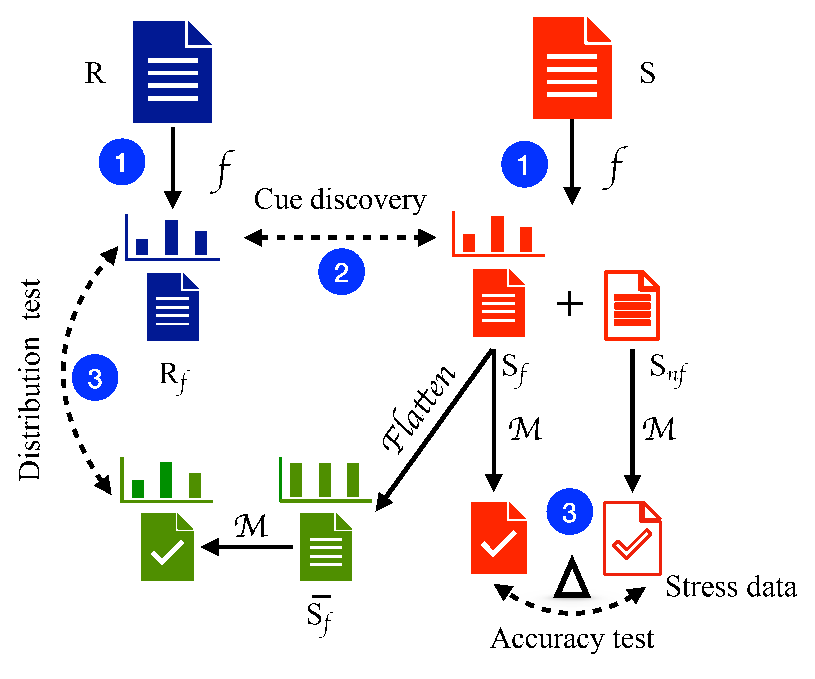
\includegraphics[width=0.8\columnwidth]{figures/emnlp/framework.eps}
\caption{ICQ工作流程。 \textcircled{1}:数据提取阶段; \textcircled{2}:线索发现阶段;
\textcircled{3}:模型探测阶段。$f$=特定特征,$R$=训练数据,$S$=测试数据,$R_f$=提取的训练数据,
$S_f$=提取的测试数据,$S_{nf}$=不包含特征$f$的剩余测试数据,$\overline{S_f}$=平衡化测试数据(flatten),$\mathcal{M}$=特定模型。}
\label{fig4:framework}
\end{figure}

我们将在下面更详细地讨论这些阶段:
\subsubsection*{1. 数据提取阶段}
\label{sec4:evaldata}
在确定了关键的语言特征之后,我们的系统首先执行的任务是构建数据提取器。对于每个特征值 \(f\),提取器的角色是处理整个数据集并识别与该特定特征值相关联的实例。具体来说,如果数据集中的某个实例包含了这个特征,那么这个实例就会被选中,并归入包含该特征的子集中。这一步是识别特征在数据集中分布和表现的基础。

\subsubsection*{2. 线索发现阶段}
\label{sec4:cuenessdiscovery}

接下来,我们针对每个特征 \(f\),将其对应的提取器应用于数据集 \(X\) 的训练和测试部分,分别标记为 \(R\) 和 \(S\),如图 \ref{fig4:framework} 所示。这导致了基于特征的实例聚类,形成了训练实例子集 \(R_f\) 和测试实例子集 \(S_f\)。一个特征被视为潜在的数据集线索,当且仅当它同时存在于训练和测试数据中。

为了计算提取集的标签分布偏差,我们使用均方误差(MSE)和Jensen-Shannon Divergence(JSD)~\cite{lin1991divergence}。线索得分反映了数据集 \(X\) 针对特征 \(f\) 的偏见程度。

均方误差(MSE)计算方法如下:
\begin{equation}
MSE(F) = \frac{1}{|\mathcal{L}|} \sum_i (y_i - \overline{y_i})^2
\end{equation}
其中,\(y_i\) 表示在提取数据集 \(F\) 中标签 \(l_i\) 的实例数,而 \(\overline{y_i}\) 是每个标签的平均实例数。较大的 \(MSE(F)\) 意味着更尖锐的标签分布,指示了更显著的偏见。

如果提取的训练集 \(R_f\) 和提取的测试集 \(S_f\) 展示出类似的偏见,那么它们分布之间的JSD将会很小。JSD的计算公式为:
\begin{equation}
JSD = \frac{1}{2}\left (Q(R_f) \parallel A \right ) + \frac{1}{2}\left (Q(S_f) \parallel A \right ),
\end{equation}
其中 \(A = \frac{1}{2}\left (Q(R_f) + Q(S_f) \right )\)。函数 \(Q()\) 表示提取数据集的标签分布。

最后,我们定义线索得分,用以衡量数据集 \(X\) 针对特征 \(f\) 的偏见程度:
\begin{equation}
cue(f, X) = \frac{MSE(R_f)}{\exp(JSD(R_f, S_f))}
\end{equation}
这个得分结合了标签分布的不均衡(MSE)和在训练与测试集之间分布的一致性(JSD),从而提供了一个全面的偏见指标。

\subsubsection*{3. 模型测试阶段 (Model Probing)}
\label{sec4:modelprobing}
在前两个结算,我们探讨了数据集 \(X\) 可能受特定线索 \(f\) 影响的可能性。
然而,关键的问题在于,基于这个数据集训练出的模型是否真的会利用这一线索。这不仅
与数据集的特性有关,而且还取决于模型的结构和训练机制。为了深入探索这一点,在第三阶段介绍
了一套框架,用于探测和评估在有偏数据集上训练的模型是否以及在多大程度上利用了特定线
索 \(f\)。此框架包括两种测试方法:准确性测试和分布测试。

\subsubsection*{准确性测试}
\label{sec4:accuracytest}
准确性测试旨在评估模型在含有和不含有特定特征 \(f\) 的数据子集上的表现差异。
这种比较能够揭示模型在面对不同数据情景时的泛化能力。具体来说,如果模型在包含特
定特征 \(f\) 的数据子集上表现更佳,这通常意味着模型已经学会利用这一特征进行预测。

在准确性测试中,我们专注于测量模型 \(M\) 在两个测试集上
的表现:一个是包含特征 \(f\) 的测试集 \(S_f\),另一个是不包含特征 \(f\) 的测
试集 \(S_{nf}\)。我们通过以下公式计算这两个测试集上准确率的差异:

\begin{equation}
\Delta Acc(f) = acc(S_f) - acc(S_{nf})
\end{equation}

这里的 \(\Delta Acc\) 值揭示了模型在处理包含和不包含特定
特征的数据子集时性能的变化。$\Delta Acc$的正值或负值表明模型在比较包含
和不包含特定特征的数据子集时性能变化的方向。正值表明模型利用该特征进行预测,
而负值则意味着模型在泛化或对该特征的敏感性上存在困难。
$\Delta Acc$的绝对值大小反映了模型性能受到特定特征存在或缺失的影响程度。
较大的绝对值表明模型更依赖或对该特征更敏感,而较小的绝对值则表明模型更健壮,
对特征的存在或缺失影响较小。


\subsubsection*{分布测试 (Distribution Test)}
\label{sec4:distributiontest}
分布测试着重于通过视觉化的方式检查特定特征的分布变化如何影响模型的预测性能。
这一测试的第一步是在提取的测试集 \(S_f\) 中创建
一个``平衡化''测试集 \(\overline{S_f}\)。我们通过平
衡化标签分布来实现这一点,即从每个标签类别中随机移除实例,直到所有
类别的实例数量相等。这一过程主要包括以下几个步骤:

\begin{itemize}
  \item 1)确定最小标签实例数量:首先检查所有标签类别的实例数量,找到其中最少
  的实例数量,这将成为我们平衡化的目标。
  \item 2)调整其他标签的实例数量:对于实例数量超过最小类别的标签,我们
  随机移除多余的实例,使其数量与最小类别相等。这一过程独立地应用于每个标签类别。
  \item 3)创建平衡化的测试集:经过上述处理,我们得到了一个每个标签实例
  数量相同的平衡化测试集。这种均衡对于后续测试至关重要,因为它确保了评
  估模型时对所有标签的公平对待。
\end{itemize}

通过这种方法,我们能够有效地评估模型对不同标签类别的处理能力,尤其是在面
对均衡分布的数据时的表现。

接下来,我们将模型应用于这个平衡化的压力测试集并获取预测结果。然后,我
们比较这些预测结果的标签分布与提取的训练数据 \(R_f\) 的标签分布。这样做的
目的是检查模型是否在预测时偏向于特定标签,尤其是当这些标签在训练数据中与特定线
索相关联时。即使测试集的输入已经被平衡处理,模型可能仍然会放大这种分布上的偏见。
我们希望通过这种比较来识别模型的潜在偏差。

综上所述,准确性测试和分布测试在评估模型对特定特征的敏感性和反应上互为补充。
分布测试专注于特征分布的变化对模型性能的影响,而准确性测试更关注模型在处理含有
和不含有特定特征的数据子集时的表现。通过结合这两种方法,我们能够从不同角度全
面评估模型对特定特征的反应。如果两种测试都显示模型对某个特征高度敏感,我们可以
更加自信地推断模型确实在利用该特征进行预测。


\subsection{实验}
\label{sec4:experiment}
在本节中,我们会首先介绍我们探究的任务和相对应的数据集,而后实验的结果和分析我们会根
据前面的方法的介绍也分成两部分,就是宏观结果分析和微观结果分析。
\subsubsection{实验数据集}

本研究的实验覆盖了12个相关的数据集,旨在涵盖两大类任务:自然语言推理分类任
务和多项选择问题。这些数据集在规模、来源、结构和挑战性方面各具特色,提供了一个全面的研究
背景。如\tabref{tab4:datasets_exp} 所示,我们展示了数据集的分类和一些实例。
\tabref{dataset_intro} 中详细列出了这12个数据集的关键特征。

\begin{table*}[th]
\centering
\includegraphics[width=\columnwidth]{figures/iconip/datasets_exp.eps}
\caption{数据集示例和归一化版本。}
\label{tab4:datasets_exp}
\end{table*}

大部分数据集基于人工编写的假设,但CQA\cite{talmor2019commonsenseqa}和
SWAG\cite{zellers2018swag}则由基于LSTM的语言模型生成。数
据集不仅在规模上不同,来源和构成方式也各有特点。部分数据集
(如STS\cite{schuster2019towards}和SWAG)引
入了对抗性实验,增添了数据多样性和挑战性。

\begin{table}[h]
\small
\centering
\begin{tabular}{lcccccc}
\toprule
\textbf{数据集} &数据大小 & 数据来源& AE& 人类表现(\%)\\ \midrule
ROC & 3.9k & CD &No &100.0 \\
COPA & 1k & CD &No &100.0 \\
SWAG & 113k & LM &Yes & 88.0\\
SNLI & 570K & CD &No &80.0\\
QNLI & 11k & CD &No &80.0\\
MNLI & 413k & CD & No &80.0\\
RACE & 100k & CD &No &94.5\\
RECLOR & 6k & CD &No &63.0\\
CQA & 12k & CD &No &88.9\\
ARCT & 2k & CD &No &79.8\\
STS& 4k & CD &Yes & - \\
Ubuntu & 100k &随机选择 & No & - \\
\bottomrule
\end{tabular}
\caption{\label{dataset_intro} 数据集中假设收集的方法。
AE = 对抗性实验, LM = 语言模型, CD = 众包, 人类表示人类在数据集上的表现。}
\end{table}


\subsubsection*{自然语言推理分类任务数据集}

在自然语言推理任务中,模型需要判断给定文本对之间的逻辑关系。本研究中包含的自然语言推理数据集有:

\begin{itemize}
    \item \textbf{SNLI}\cite{bowman2015large}:拥有570K个实例,通过人类标注构建而成,旨在测试模型理解自然语言的能力。
    \item \textbf{QNLI}\cite{wang2018glue}:含有11K个问题-答案对,主要通过众包方式收集,挑战模型在问题回答方面的性能。
    \item \textbf{MNLI}\cite{williams2018broad}:具有413K个实例,也是通过众包方式构建,用以评估模型在不同文体和话题上的推理能力。
\end{itemize}

这些数据集的共同点在于它们都要求模型从给定的前提和假设中推断出正确的结论。

\subsubsection*{多项选择问题数据集}

多项选择问题要求参与者(或模型)从多个选项中选择一个正确答案。本研究涉及的相关数据集包括:
\begin{itemize}
    \item \textbf{ROC}\cite{mostafazadeh2016corpus} 
    和 \textbf{COPA}\cite{roemmele2011choice}:分别包含3.9K和1K个实例,这些数据集主要通过众包方式收集,用于评估模型在故事理解和因果推理方面的能力。
    \item \textbf{SWAG}(含113K实例)和 \textbf{Ubuntu}\cite{lowe2015ubuntu}(包含100K实例):分别由基于LSTM的语言模型和随机选择方式生成,用于测试模型在生成连贯性和上下文理解方面的性能。
    \item \textbf{RACE}\cite{lai2017race}(含100K实例)、\textbf{RECLOR}\cite{yu2020reclor}(含6K实例)、\textbf{CQA}(含12K实例)、
    \textbf{ARCT}\cite{habernal2018argument}(含2K实例)及 \textbf{STS}(含4K实例):这些数据集通过众包方式收集,每个都提供独特的挑战,如文本理解、逻辑推理和论证分析。
\end{itemize}

\subsubsection{宏观结果分析}
\label{sec4:experiment1}
我们进行了实验,以展示我们框架在两个方面的有效性:
首先,我们应用我们的方法来检测线索,6种不同任务的12个\textbf{数据集}(\tabref{tab4:datasets_exp}所示)中量化信息泄露量。
其次,我们评估了一些流行的NLP\textbf{模型}在被分为简单和困难两部分的原始测试集上的真实推理能力。

\subsubsection*{1. 数据集线索检测效果评估}
我们的线索检测效果评估实验分为以下部分:量化信息泄露的方法论、线索评估技术和度量标准、与数据集中偏差的揭示。
\subsubsection*{量化信息泄露的方法论}

在本研究中,我们专注于量化数据集中信息泄露或偏差的程度。为此,我
们开发了一种新的度量标准,命名为 $\mathcal{D}$,其定义
为 $\mathcal{D} = \text{Acc} - \text{Majority}$。在这个
公式中,$\text{Acc}$ 表示模型仅基于虚假线索的准确率,而 $\text{Majority}$ 代表通过
多数投票机制得到的准确率。

这一度量标准的核心在于评估和比较两种不同情境下的准确率,从而揭示数据集中
存在的潜在线索。具体来说:

\begin{itemize}
  \item \textbf{$\mathcal{D}$ 的高绝对值}:这意味着数据集中存在大量的线索,这些线索可能被模型用来做出预测。换句话说,如果 $\mathcal{D}$ 的值很高,这通常指示数据集中存在明显的信息泄露问题,可能导致模型偏向于特定的线索,而不是学习到更深层次的、真实的推理模式。
  \item \textbf{$\mathcal{D}$ 的低值}:较小的 $\mathcal{D}$ 值并不直接指示偏差较少,而是可能意味着训练和测试数据之间的信息``泄露''较少。这可以被解释为模型不过度依赖于数据集中的特定线索,从而可能展现出更加均衡和泛化的学习能力。
  \item \textbf{$\mathcal{D}$ 值的正负}:如果 $\mathcal{D}$ 为正,这表明模型在预测时正在利用这些线索。它为研究者提供了一个有力的工具,用于判断模型是否在依赖数据集中的特定信息,而非进行真实的、基于内容的推理。
\end{itemize}

这种方法论的通用性使其适用于评估任何多项选择类型的数据集。通过应用这一
度量标准,我们能够有效地识别和量化不同数据集中的信息泄露问题,从而为进一步的
分析和改进提供了坚实的基础。

\subsubsection*{线索评估技术和度量标准}

%\subsection*{综合评估方法的选择}
为了深入探究我们研究中的线索检测效果,我们采用了一种核心技术——``仅假设方法'',
将其作为评估虚假线索存在的标准。这种方法独特之处在于,它仅考虑假设部分的信息,
而不涉及问题的前提。通过这种方式,如果模型仅凭假设就能准确预测答案,这可能揭示
了数据集中的偏见或泄露。

%\subsection*{方法的简化与实施}
进一步地,为了简化评估过程并寻找类似于``仅假设方法''的有效度量,我
们实施了四种更为简单的方法:平均值分类器(Ave)、最大值分类器(Max)、随机
梯度下降分类器(SGDC)和逻辑回归(LR)。这些方法基于不同逻辑,旨在从不同角
度评估和解释数据集中的线索。这些方法在~\ref{sec4:approach1}中详细阐述

%\subsection*{线索类型的分析}
我们的方法与``仅假设方法''最显著的区别在于依赖的线索类型。我
们的方法着重于可解释的、基于词汇的线索,相比之下,``仅假设方法''则涉
及更复杂、不易解释的线索。这种差异不仅揭示了我们方法的独特性,也强调了
我们在方法选择上的多样性。

%\subsubsection对比``仅假设模型''}
%
%\subsection*{实验设计的考量}
我们的研究主要关注于\textbf{评估和验证我们提出的偏差检测方法}。这种方法的核心在于与传统的基于仅假设模型的表现进行对比分析。
我们的目标是证明我们的方法在识别多项选择数据集中的虚假统计线索方面的有效性,
进而彰显我们所做工作的贡献。

在这一实验框架下,我们采用了皮尔逊相关系
数(Pearson Correlation Coefficient, PCC)来衡量我们的
方法与已有的仅假设模型之间的相似度。这里,我们特别关注了FastText和BERT这两种
模型。我们的分析覆盖了12个不同的数据集,并运用了八种线索分数度量方法和四种聚合算法。

分析结果,如表\ref{best_method}所展示的,突出表明了
在所有12个数据集中,CP线索分数与逻辑回归模型的结合展示出与仅假设
模型(例如FastText和BERT)高度的相关性。与FastText和BERT模型相比,我
们的方法在PCC得分上分别达到了97.17%和97.34%。这些显著的结果使我们得
出结论,CP线索分数和逻辑回归模型的结合为评估所有数据集提供了一种强有力的方法。
%为了详细了解这些数据,可以参考附录中的完整信息。

\begin{table}[th]
\scriptsize
\centering
\setlength{\tabcolsep}{3pt}
\begin{tabular}{cccc|ccc|ccc|ccc}
\toprule
     & \multicolumn{3}{c|}{Ave}      & \multicolumn{3}{c|}{Max}      & \multicolumn{3}{c|}{SGDC}       & \multicolumn{3}{c}{LR}     \\ \midrule
     & FT & BERT & P     & FT & BERT & P     & FT & BERT & P     & FT & BERT & P     \\ \midrule
PMI  & 90.87       & 96.23   & 93.55 & 95.37       & 79.82   & 87.59 & 97.81       & 91.01   & 94.41 & 97.14       & 96.05   & 96.6  \\
LMI  & 65.13       & 49.18   & 57.16 & 34.52       & 30.71   & 32.62 & 69.88       & 79.06   & 74.47 & 77.46       & 81.21   & 79.33 \\
AD   & 84.62       & 72.49   & 78.56 & 90.75       & 73.02   & 81.89 & 93.73       & 76.24   & 84.98 & 97.56       & 86.91   & 92.24 \\
WP   & 86.87       & 73.09   & 79.98 & 92.47       & 79.87   & 86.17 & 94.0        & 22.59   & 56.53  & 61.28       & 75.55   & 65.86 \\
RD   & 96.59       & 93.82   & 95.21 & 98.23       & 91.04   & 94.63 & 94.30       & 93.98   & 94.14 & 94.21       & 95.59   & 94.90 \\
Cos  & 94.84       & 82.94   & 88.89 & 92.73       & 75.40   & 84.07 & 98.08       & 87.86   & 92.97 & 87.38       & 78.44   & 82.91 \\
Freq & 68.00       & 50.02   & 59.01 & 34.45       & 30.67   & 32.56 & 64.08       & 67.11   & 65.60 & 74.58       & 88.64   & 81.61 \\
CP   & 93.09        & 96.61   & 94.85 & 95.29       & 79.80   & 87.54 & 97.19       & 96.16   & 96.67 & 97.17       & 97.34   & \textbf{97.26} \\ 
\bottomrule
\end{tabular}
\caption{\label{best_method} 在12个数据集上,我们的方法的$\mathcal{D}$与FastText和BERT的``仅假设''模型的$\mathcal{D}$之间的皮尔逊分数。其中,P表示BERT和FastText(简称FT)的平均皮尔逊相关系数。}
\end{table}

基于这些发现,我们坚信基于CP的方法是一种强大的工具,能够识别数据集中的关键词特征。这是通过计算
我们在\ref{sec4:approach1}章节中描述的``线索度''来实现的。
此外,CP线索和逻辑回归模型的结合为确定多项选择数据集受信息泄露影响的
程度提供了一个有效的度量标准,这对于我们的研究领域来说是一个重要的贡献。

此外,我们通过绘制偏差分数$\mathcal{D}$,来可视化我们的发现,
并对我们的CP+LR方法与两种仅假设
模型(FastText和BERT)在12个数据集上的表现进行
了比较,如\figref{fig4:d_figure}所示。图中的线条的一致性显示了我们
的方法与仅假设模型之间的强相关性。

\begin{figure}[th]
    \centering
    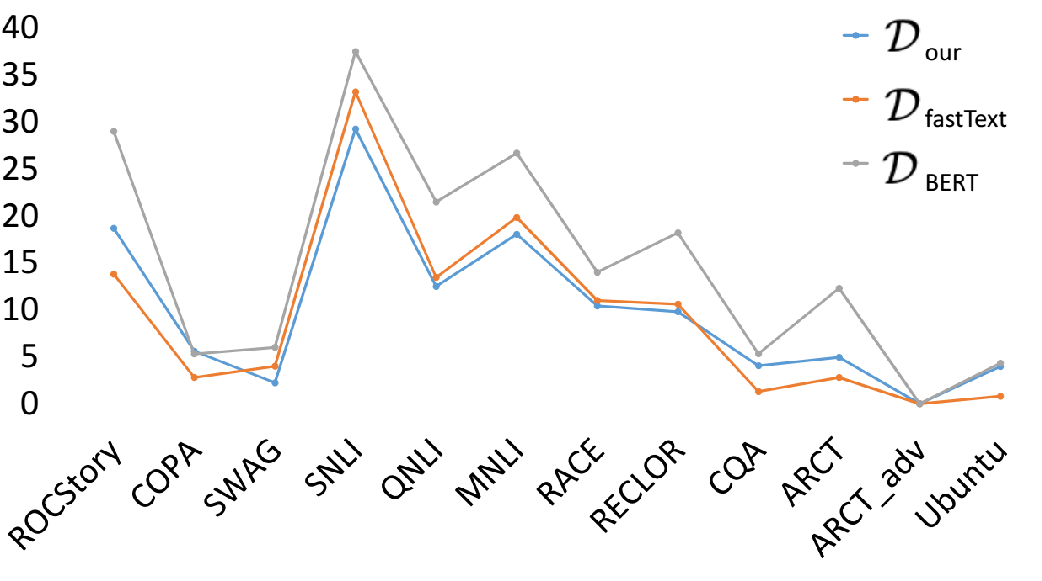
\includegraphics[width=0.65\columnwidth]{figures/iconip/d_figure.pdf}
    \caption{所有12个数据集上三种预测模型的偏差分数。}
    \label{fig4:d_figure}
    \end{figure}
综上所述,我们的方法有效地识别并量化了数据集中的偏差,并且与
仅假设模型的高度相关性进一步证明了我们方法的有效性和合理性。

\subsubsection*{数据集中偏差的揭示}
\textbf{为了更准确地识别那些存在问题的数据集},我们基于实验结果制定了一套详尽的标准。这
套标准的核心在于,如果一个模型在任何给定的线索特征上的偏差$\mathcal{D}$超
过10\%,我们就认定该数据集存在显著问题。这一简洁的评判标准使我们能迅速
辨认出那些含有严重统计线索问题的数据集。

在表\ref{tab4:best_acc}中,我们展示了四种简单分类模型在12个不同数据集上的最
高准确率,以及与多数选择(Majority)的偏差。这一表格详尽记录了使用词语线索
特征时,在各数据集上的选择结果。


\begin{table}[th]
    \small
    \centering
    \begin{tabular}{lcccccc}
    \toprule
    \textbf{数据集} &多数选择 & \multicolumn{2}{c}{Word Cues}  \\ \midrule
                                         & (\%)                 &  Acc.(\%) & $\mathcal{D}(\%)$ \\ \midrule
    ROC & 50.0            & 68.68          & \textbf{18.68}   \\
    COPA        & 50.0           & 55.60           &  5.60                \\
    SWAG       & 25.0           & 27.23           &   2.23                \\
    SNLI          & 33.33      & 62.57           &  \textbf{29.24}      \\
    QNLI         & 50.0           & 62.49            &  \textbf{12.49}   \\
    MNLI         & 33.33      & 51.37            &\textbf{18.04}        \\
    RACE        & 25.0          & 35.42            &   \textbf{10.42}   \\
    RECLOR       & 25.0           & 34.80            &   9.80   \\
    CQA          &20.0            & 23.42            &  3.42      \\
    ARCT        & 50.0            & 54.95           &  4.95      \\
    STS& 50.0           &50                 &0.0      \\
    Ubuntu   & 1.0               &4.96              &3.96      \\
    \bottomrule
    \end{tabular}
    \caption{\label{tab4:best_acc} 我们的四种简单分类模型在12个数据集上的最高准确率和与多数选择的偏差。}
    \end{table}

根据这个标准,我们识别出ROCStories、SNLI、MNLI、QNLI、RACE和RECLOR等
数据集存在大量统计线索问题。如表所示,这些数据集中的$\mathcal{D}$值显著高
于10\%的阈值,表明它们包含大量可以被模型利用的虚假统
计线索。例如,在ROCStories数据集中,我们的方法实现的最高准确率比随机选择高
出20.92\%,而在SNLI数据集中,这一比例甚至高达33.59\%。这进一步证明了这些数据集中存在的问题。

另外,我们也观察到,在未经过对抗性过滤且受到人为干预的数据集,例如
ARCT,存在更多的虚假统计线索。在对ARCT数据集进行的人工调整中
,我们发现准确率有显著变化(从54.95\%降至50\%),这表明人为干预对数据集质量的影响。
    
综上所述,在表格中我们报告了四种简单分类模型在12个数据集上的最高准
确率以及与多数选择的偏差。我们的发现表明,偏差$\mathcal{D}$是一个有效的工具,可
以用来识别和评估数据集中存在的词语线索问题。

总的来说,我们对问题数据集的深入分析和标准化方法,能够帮
助研究人员识别出含有大量统计线索问题的数据集。这一关键洞见将有
助于发展更加健壮的模型,使其不那么依赖于表面的统计线索,而是能够更深入地理解和处理复杂的数据。


\subsubsection*{2. 模型推理能力的评估}

\textbf{为了探究模型是否学习了数据集中的线索特征},并因此做出有偏见的选择,
本研究提出了一种方法来评估模型是否受到数据集中线索的影响。我们假设,
如果一个模型确实受到这些线索的影响,那么它在简单和困难部分的表现将会有所不同。
这种表现上的差异被称为\textbf{性能差距},它反映了模型的健壮性。
一个健壮的模型,理论上应当对虚假信息不敏感,并在简单和困难两部分的测试中
表现出类似的性能。尤其是在困难部分的表现,是衡量模型能力的一个重要指标。

%表\ref{tab4:gap_acc}展示了三种不同的模型——BERT、ESIM和FastText——在六个数据集上的
%性能差距。表格中的数据显示了这些模型在简单和困难测试部分上的表现差异,突出
%了各模型对线索特征的敏感程度。

\begin{table}[th]
    \small
    \centering
    \begin{tabular}{ccllll}
    \toprule
    数据集                                     & \multicolumn{1}{c}{模型} & \multicolumn{1}{c}{原始测试} & \multicolumn{3}{c}{线索分类}                                                                                        \\ \midrule
                                                 &                            & \multicolumn{1}{c}{(\%)}      & \multicolumn{1}{c}{简单} & \multicolumn{1}{c}{困难} & \multicolumn{1}{c}{\textbf{差距}} \\ \midrule
    \multicolumn{1}{c}{\multirow{3}{*}{SNLI}}   & BERT                       & \multicolumn{1}{l}{90.48}    & 94.99                         & 83.02                         & 11.97                         \\
    \multicolumn{1}{c}{}                        & ESIM                       & \multicolumn{1}{l}{87.44}    & 93.27                         & 77.77                         & 15.50                         \\
    \multicolumn{1}{c}{}                        & FastText                   & \multicolumn{1}{l}{54.74}    & 73.16                         & 24.23                         & 48.93                        \\ \midrule
    \multicolumn{1}{c}{\multirow{3}{*}{MNLI}}   & BERT                       & \multicolumn{1}{l}{85.10}    & 90.60                         & 79.30                         & 11.30        \\
    \multicolumn{1}{c}{}                        & ESIM                       & \multicolumn{1}{l}{76.82}    & 85.80                         & 67.34                         & 18.46                    \\
    \multicolumn{1}{c}{}                        & FastText                   & \multicolumn{1}{l}{47.15}    & 66.88                         & 26.31                         & 40.56                    \\ \midrule
    \multicolumn{1}{c}{\multirow{3}{*}{QNLI}}   & BERT                       & \multicolumn{1}{l}{88.89}    & 90.92                         & 85.54                         & 5.37             \\
    \multicolumn{1}{c}{}                        & ESIM                       & \multicolumn{1}{l}{72.17}    & 78.55                         & 61.66                         & 16.89                \\
    \multicolumn{1}{c}{}                        & FastText                   & \multicolumn{1}{l}{66.33}    & 80.94                         & 42.26                         & 38.67                 \\ \midrule
    \multicolumn{1}{c}{\multirow{3}{*}{ROC}}    & BERT                       & \multicolumn{1}{l}{90.54}    & 93.53                         & 84.01                         & 9.52             \\
    \multicolumn{1}{c}{}                        & ESIM                       & \multicolumn{1}{l}{65.42}    & 72.49                         & 50.00                         & 22.49                  \\
    \multicolumn{1}{c}{}                        & FastText                   & \multicolumn{1}{l}{62.91}    & 71.16                         & 44.90                         & 26.26                 \\ \midrule
    \multicolumn{1}{c}{\multirow{3}{*}{RACE}}   & BERT                       & \multicolumn{1}{l}{90.54}    & 93.53                         & 84.01                         & 9.52                           \\
    \multicolumn{1}{c}{}                        & ESIM                       & \multicolumn{1}{l}{65.42}    & 72.49                         & 50.00                         & 22.49                       \\
    \multicolumn{1}{c}{}                        & FastText                   & \multicolumn{1}{l}{62.91}    & 71.16                         & 44.90                         & 26.26                        \\ \midrule
    \multicolumn{1}{c}{\multirow{3}{*}{RECLOR}} & BERT                       & \multicolumn{1}{l}{48.40}    & 61.68                         & 41.74          & 19.93         \\
    \multicolumn{1}{c}{}                        & ESIM                       & \multicolumn{1}{l}{40.40}    & 52.69                         & 34.23                         & 18.46                 \\
    \multicolumn{1}{c}{}                        & FastText                   & \multicolumn{1}{l}{31.60}    & 43.11                         & 25.83                         & 17.29                          \\ 
    \bottomrule
    \end{tabular}
    \caption{\label{tab4:gap_acc} 模型在简单和困难测试数据集上的性能差距(\%)。}
    %模型捕捉单词的分布分数作为线索特征进行决策。}
    \end{table}

我们评估了3个典型的模型——BERT~\cite{devlin2018bert}、ESIM~\cite{chen2017enhanced}和FastText~\cite{joulin2017bag}——在6个``差''数据集上的表现,分别代表不同的复杂性层级:

\textit{FastText}: 这个模型将句子视为n-gram的集合,并试图独立预测每个答案的正确概率。在
这个模型中,单词的表示是基于300维的GloVe嵌入。在多项选择的设置中,FastText选择
得分最高的答案作为预测结果。由于其简单的结构,FastText在处理文本时可能更依赖于表
面的词汇特征,这可能导致在复杂的推理任务中性能不足。

\textit{ESIM}: 这个模型通过引入局部推理建模来增强其性能。它在两个片段局部对齐后,对前提和假
设之间的推理关系进行建模。我们使用GloVe嵌入对自己的ESIM模型进行训练,并选择得分最高
的答案。ESIM通过在前提和假设之间建立更复杂的关系来处理任务,这使其在处理需要深层次理
解的任务时表现更好。

\textit{BERT}:BERT模型基于Transformer架构,这是目前深度学习领域非常流行的一种结构。它的训练是在两个无监督的任务上进行的,
这两个任务分别是:遮蔽语言模型(MLM)和下一句预测(NSP)。这些
训练是在BooksCorpus和英文维基百科的文本上完成的。有多种预训练的
BERT模型可用,它们在层数和参数数量上有所不同。我们选择的是一
个基础版本,具有12层Transformer块、768个隐藏单元和12个自注意力头,共计110M个参数。
BERT对前提和假设的连接(带有分隔符)进行了3个周期的微调,以预测基于前提和假设的关系。
BERT的这种架构使其能够在处理需要广泛上下文理解和复杂推理的任务时表现出色。


这些模型在不同数据集上的表现及其在简单和困难部分之间的差距如\tabref{tab4:gap_acc}所示。简单和困难部分之间的差距通常在10-50%之间。
相比之下,人类在困难集上仍然能够保持良好的表现,这表明这些模型可能在某种程度上都受到了各自数据集中统计线索的影响。``组合''意味着我们汇总了由词语线索做出的选择。
对于``组合''而言,简单部分是其他两个线索特征简单部分的并集,而困难部分是两个其他困难部分的交集。我们发现``组合''通常会导致更大的差距。

在对比三个模型的性能差距时,我们发现BERT、ESIM和FastText的差距依次增大。
例如,FastText在SNLI数据集上的性能差距高达48.93\%,而BERT为11.97\%。这表明BERT可能
比其他两个模型更具健壮性。然而,所有模型在六个数据集上的性能差距均超过了10\%,这暗示
即便是BERT也受到了数据集中线索的影响。

值得注意的是,最高分数的模型并不总是最稳定的。例如,在RACE和RECLOR数据
集上,尽管BERT的整体准确率更高,但它的性能差距比其他模型更大。ESIM在RACE
上的差距相对较小,但考虑到其在困难测试数据上的表现接近随机选择,我们不能简
单地认为ESIM更优。此外,ESIM在RACE和RECLOR数据集上表现出较大的收敛困难。

综合来看,我们提出了一种新的模型评估方法,即通过困难数据测试来考察模型的准确率和
健壮性。通过性能差距分析,我们可以深入理解模型的局限性,并努力改进它们。通过减少性
能差距,我们可以开发出即使在具有挑战性情境下也能保持高性能的更健壮模型。

\subsubsection{微观结果分析}
\label{sec4:experiment2}


\begin{table}[htbp]
   \centering
    \scriptsize
    \begin{tabular}{p{0.09\textwidth}
    >{\centering}p{0.10\textwidth}
    >{\centering}p{0.08\textwidth}
    >{\centering}p{0.08\textwidth}
    >{\centering}p{0.08\textwidth}
    >{\centering}p{0.08\textwidth}
    c}
    \toprule
    数据集 & Top Cues & Cueness & FT  & ES & BT & RB\\ 
        &	& \%	& ($\Delta$)& ($\Delta$)& ($\Delta$)& ($\Delta$) \\ \hline
    \multirow{5}{*}{SNLI} 
    & ``sleeping'' & 13.95 & 30.3 &6.81 & 5.34& 4.87 \\                                                                    
    & ``no'' & 13.33 & 18.09 &3.32 & 2.05& 2.6 \\
    & ``because'' & 9.24 & 18.89 &4.88 & 5.61& 4.31 \\
    & ``friend'' & 8.82 & 22.96 &6.66 & 3.51& 3.05 \\
    & ``movie'' & 7.73 & 16.64 &0.06 & 9.47& -0.19 \\
           \midrule 
    \multirow{5}{*}{QNLI} 
    & ``dioxide'' & 4.52 & 9.78 &-0.06 & 4.97& 10.56 \\                                                                    
    & ``denver'' & 4.26 & 13.59 &7.14 & 2.23& 3.11 \\
    & ``kilometre'' & 4.24 & 4.85 &6.43 & 4.67& 2.55 \\
    & ``mile'' & 3.95 & 7.16 &15.64 & -1.65& -6.65 \\
    & ``newcastle'' & 3.8 & 3.44 &12.0 & 0.89& -1.23 \\
           \midrule 
    \multirow{5}{*}{MNLI} 
    & ``never'' & 10.4 & 29.15 &26.41 & 9.86& 10.6 \\                                                                      
    & ``no'' & 8.98 & 19.49 &20.17 & 1.2& 3.32 \\
    & ``nothing'' & 8.98 & 25.5 &26.84 & 5.11& 4.32 \\
    & ``any'' & 6.79 & 20.4 &19.39 & 7.76& 3.74 \\
    & ``anything'' & 5.73 & 18.43 &15.74 & 3.31& 1.14 \\
           
    \midrule 
    \multirow{5}{*}{ROC} 
    & ``threw'' & 12.99 & 1.28 &4.69 & 10.88& 0.97 \\                                                                      
    & ``now'' & 8.68 & -10.01 &14.51 & 1.75& 5.69 \\
    & ``found'' & 8.16 & -2.31 &4.45 & 5.12& -3.13 \\
    & ``won'' & 7.71 & 2.43 &0.74 & 1.05& 5.51 \\
    & ``like'' & 7.3 & 4.77 &10.06 & 8.81& 1.67 \\
           \midrule 
    \multirow{5}{*}{COPA} 
    & ``went'' & 3.61 & -10.83 &6.46 & 7.92& 1.04 \\                                                                       
    & ``got'' & 2.74 & 5.45 &-9.89 & -12.52& -10.3 \\
    & ``for'' & 2.14 & 10.11 &-1.89 & 9.05& 11.58 \\
    & ``with'' & 1.38 & -15.64 &-6.98 & 3.3& 13.82 \\
    & TYPO & 0.84 & -12.46 &-2.33 & 3.8& -8.22 \\
           \midrule 
    \multirow{5}{*}{SWAG}
    & ``football'' & 7.38 & 6.13 &8.55 & 1.2& 1.55 \\
    & ``anxious'' & 6.65 & 7.55 &-4.67 & -6.66& -1.67 \\
    & ``concerned'' & 6.19 & 12.6 &4.58 & 8.27& -5.66 \\
    & ``skull'' & 5.73 & -2.77 &0.49 & 8.43& 3.49 \\
    & ``cop'' & 5.01 & 2.79 &5.3 & -0.92& -0.04 \\
           \midrule 
    
    \multirow{5}{*}{RACE} 
    & ``above'' & 13.74 & 8.73 &-8.43 & -0.22& -1.92 \\                                                                    
    & ``b'' & 12.84 & 16.97 &-4.8 & 3.52& -3.45 \\
    & ``c'' & 11.83 & 15.69 &-6.94 & 8.6& -7.6 \\
    & ``probably'' & 6.77 & 9.91 &-0.06 & -3.8& 2.86 \\
    & ``may'' & 4.2 & 7.75 &-3.45 & -6.67& -1.8 \\
           
           \midrule 
    \multirow{5}{*}{RECLOR} 
    & ``over'' & 2.07 & 1.76 &-2.94 & -1.35& -4.12 \\                                                                      
    & ``result'' & 1.97 & -3.29 &-2.69 & -1.78& -3.7 \\
    & ``explanation'' & 1.81 & -6.33 &-1.73 & -2.76& -7.24 \\
    & ``proportion'' & 1.68 & -5.64 &-4.69 & 2.37& -2.16 \\
    & ``produce'' & 1.4 & 4.54 &-2.98 & -14.36& -3.7 \\
           \midrule 
    \multirow{5}{*}{ARCT} 
    & ``not'' & 3.74 & -2.54 &7.45 & -0.97& -11.96 \\                                                                      
    & NEGATION & 2.85 & 3.49 &10.04 & 6.28& -8.23 \\
    & ``n't'' & 2.52 & 10.3 &5.89 & 9.49& 4.84 \\
    & ``always'' & 2.25 & -4.66 &38.21 & -4.35& -8.26 \\
    & ``doe'' & 2.06 & -0.73 &-3.69 & -1.15& -7.22 \\
           \midrule 
    STS& OVERLAP & 1.96e-10 & 1.65 &-0.25 & 2.73& 0.57 \\ \midrule
    \multicolumn{3}{c|}{$\sum(|.|)$ (Model weakness)} 	& 469.8 & 361.4 & 227.7 & 216.2 \\
    \bottomrule 
    \end{tabular}
    \caption{数据集、每个数据集的前5个线索和每个模型在这些线索上的准确率偏差$\Delta$。}
    \label{tab4:bias}
    \end{table}
    %\clearpage
    在节中,我们将重点讨论关于线索发现、
模型探测和分析的成果以及有关ChatGPT模型评估的案例分析。
这一整套框架已经在我们的在线演示中得到实现和展示。

\subsubsection*{1. 数据集中的线索发现} 

我们利用在\secref{sec4:approach2}中描述的方法,对不同数
据集中的线索进行了识别和分析。具体来说,我们首先运用本研究定义的各种特征,
对每个数据集的训练和测试数据进行筛选。在\tabref{tab4:bias}的左半部分,我们展示了每个
数据集中发现的前五个主要线索及其相应的线索得分。

以STS数据集为例,这是一个经过精心平衡的对抗性数据集,我
们在其中只识别出一个线索——OVERLAP,且该线索的得分非常低。这一发现并不出
乎意料,因为OVERLAP作为我们列出的特征中唯一涉及前提和假设标记的``二阶''特征
,很可能已经避开了数据创建者创造的偏见。

在大多数情况下,我们发现的主要线索都是词汇特征。除了OVERLAP之外,
我们还在列表中发现了如NEGATION和TYPO等特征。有趣的是,当我们将关注
的线索扩展到前十个时,情感(SENTIMENT)和命名实体识别(NER)特征也显
现出来。值得注意的是,我们还发现了一些以往其他研究报告中提到的、被认为
有偏见的特征,比如ARCT中的``not''和NEGATION,MNLI和SNLI中的``no'',以
及ROC中的``like''。尤其在MNLI数据集中,我们发现所有五个识别出的线索都与负
面词汇相关,这表明该数据集可能包含了显著的人为痕迹,从而可能导致模型的脆弱性。

此外,我们还注意到某些词汇线索揭示了问题中的特定句法、语义或情感模式。例如,SNLI
数据集中的``because''表明了因果关系的存在;ROC中的``like''通常与积极情感相关
;RACE中的``probably''和``may''表达了不确定性等。这些发现可作为修订数据集时的重要线索。

\subsubsection*{2. 模型偏见的探测和分析}
为了深入探索模型是否受到数据集中特定线索或特征的影响,我们在
原始训练集上对四种模型——FastText、ESIM、BERT和RoBERTa——进行了训练。与
之前的宏观测试相比,我们新增了RoBERTa模型的研究。作为BERT的改进版本,RoBERTa通过
在更大的数据集上训练、增加批量大小,并去除了一些原始BERT的目标,例如下一句预测(NSP),从
而显著提高了性能。这些改进使得RoBERTa在多种自然语言处理任务上表现更加出色。我们选用的
是RoBERTa的基础版(base version)进行测试。接下来,我们通过准确性和分布测试来评估这些模型。

\subsubsection*{准确性测试}
我们在\tabref{tab4:bias}中展示了测试结果。如\ref{sec4:accuracytest}所
述,$\Delta$值的正负号表示模型在含有和不含特定特征的数据子集之间性能变化的方
向。$\Delta$的绝对值大小则反映了模型性能受这些特征影响的程度。较大的$\Delta$值表
明模型对特定特征有更强的依赖或敏感性,而较小的值则意味着模型更加健壮。

在\tabref{tab4:bias}的底部,我们观察到,跨越所有十个
数据集,$\Delta$绝对值的总和遵循以下顺序:RoBERTA $<$ BERT $<$ ESIM $<$ FastText。这
与我们之前的假设和社区对这些模型的普遍看法一致。然而,对单个数据集和特征的细致检查揭示
了更复杂的情况。例如,FastText倾向于捕捉单词级的线索,而不是深层次的语义线索,而像BERT和
RoBERTa这样的更复杂模型则对结构性特征(如NEGATION和SENTIMENT,实际上是词汇类别)更
敏感。这种差异可以通过FastText的设计理念来解释,它更专注于单词层面,而不是句法或语义结构。

有趣的是,FastText对TYPO特征显示出了强烈的负相关性。我们推测,这可能是因
为FastText使用了更规范的词汇进行训练,因此对于文本中的拼写错误表现出了较低的容忍度。

\subsubsection*{分布测试}
\begin{figure}[th]
    \centering
    \begin{minipage}[b]{0.45\linewidth}
    \centering
    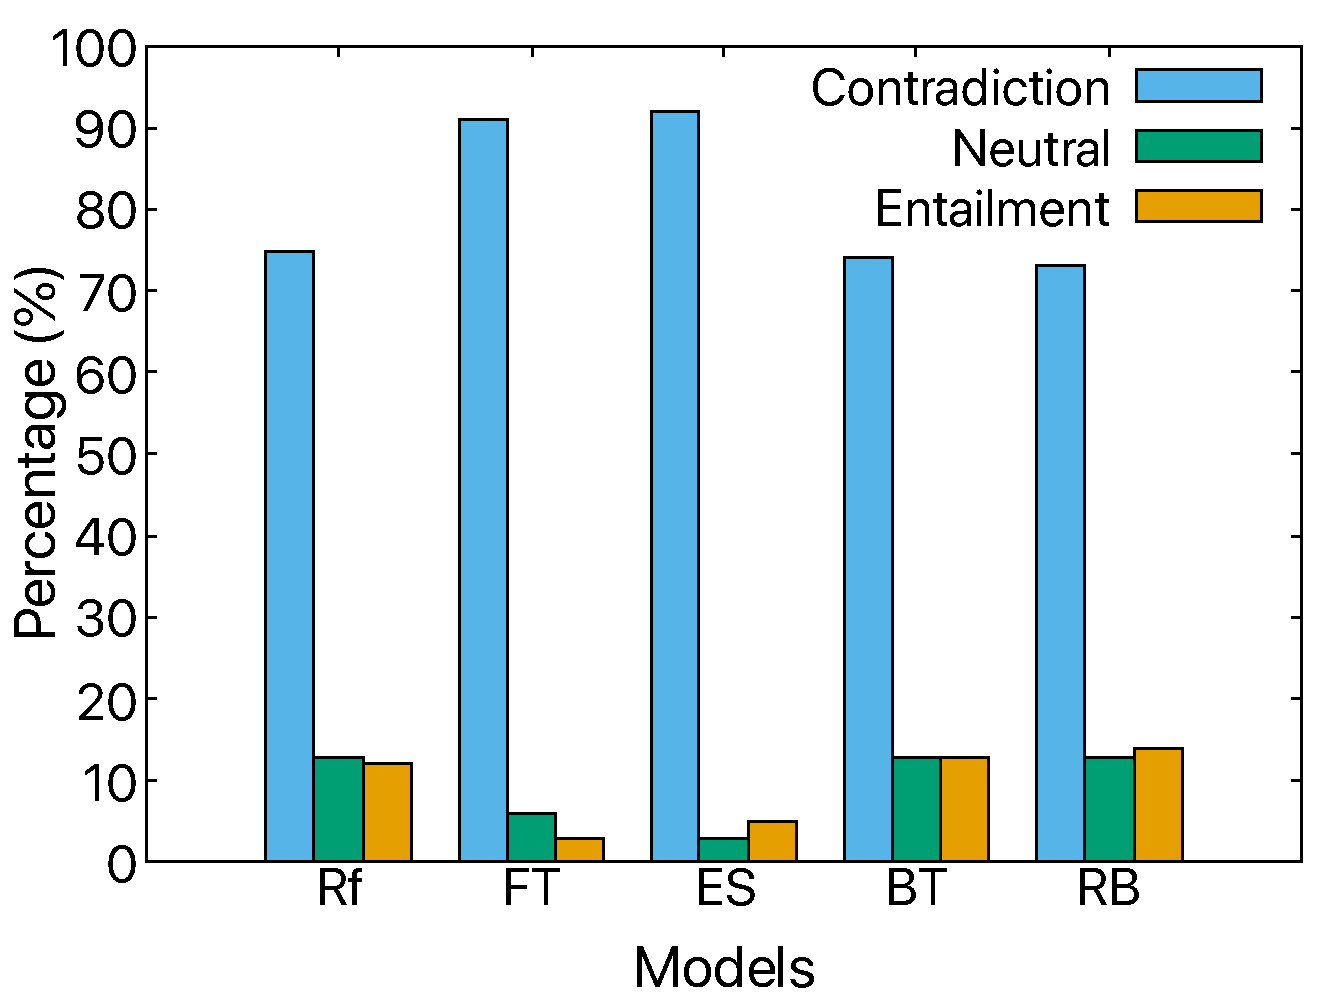
\includegraphics[width=\columnwidth]{figures/emnlp/no-mnli.pdf}
    \caption*{MNLI中的线索``no''} 
    \label{fig4:cue_no} 
    \end{minipage}
    \hspace{0.5cm} 
    \begin{minipage}[b]{0.45\linewidth} 
    \centering 
    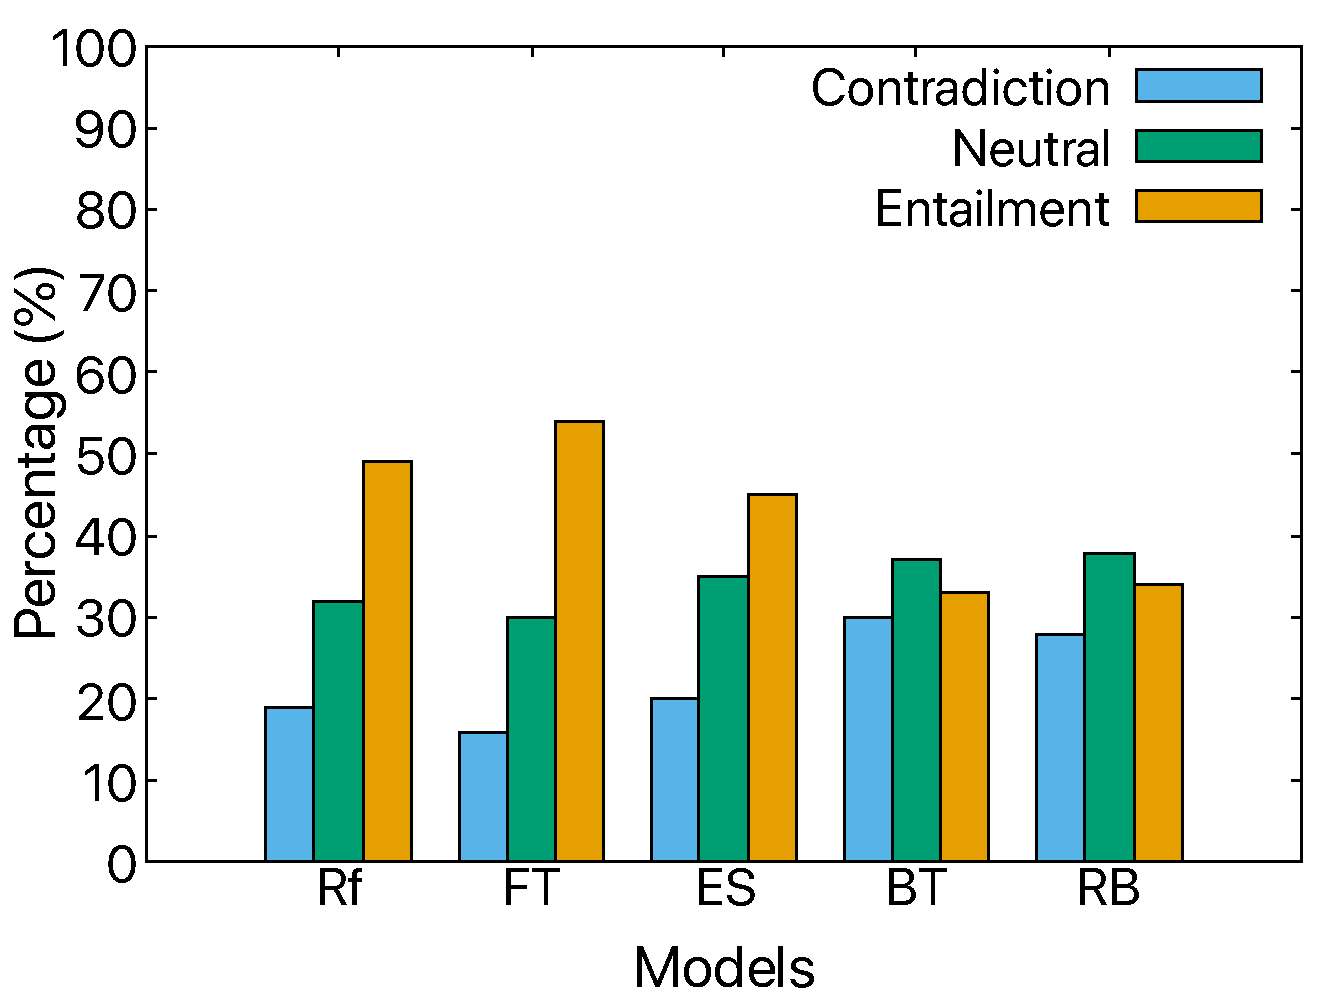
\includegraphics[width=\columnwidth]{figures/emnlp/speaking-snli.pdf} 
    \caption*{SNLI中的线索``speaking''}
    \label{fig4:cue_speaking}
    \end{minipage}
    
    \vspace{0.5cm}
    
    \begin{minipage}[b]{0.45\linewidth}
    \centering
    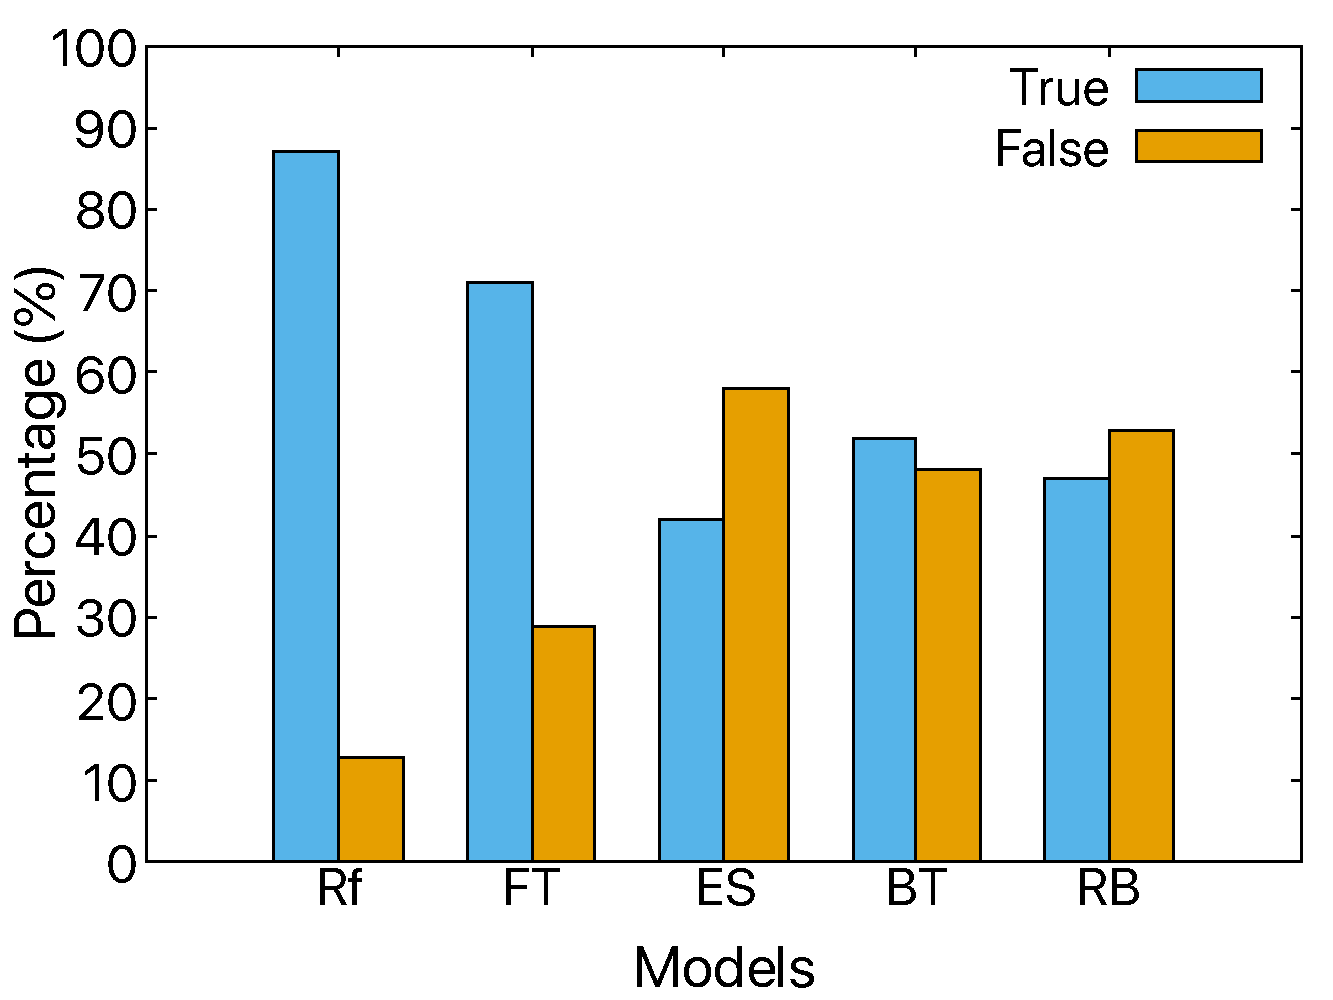
\includegraphics[width=\columnwidth]{figures/emnlp/above-arct.pdf}
    \caption*{ARCT中的线索``above''} 
    \label{fig4:cue_above} 
    \end{minipage}
    \hspace{0.5cm} 
    \begin{minipage}[b]{0.45\linewidth} 
    \centering 
    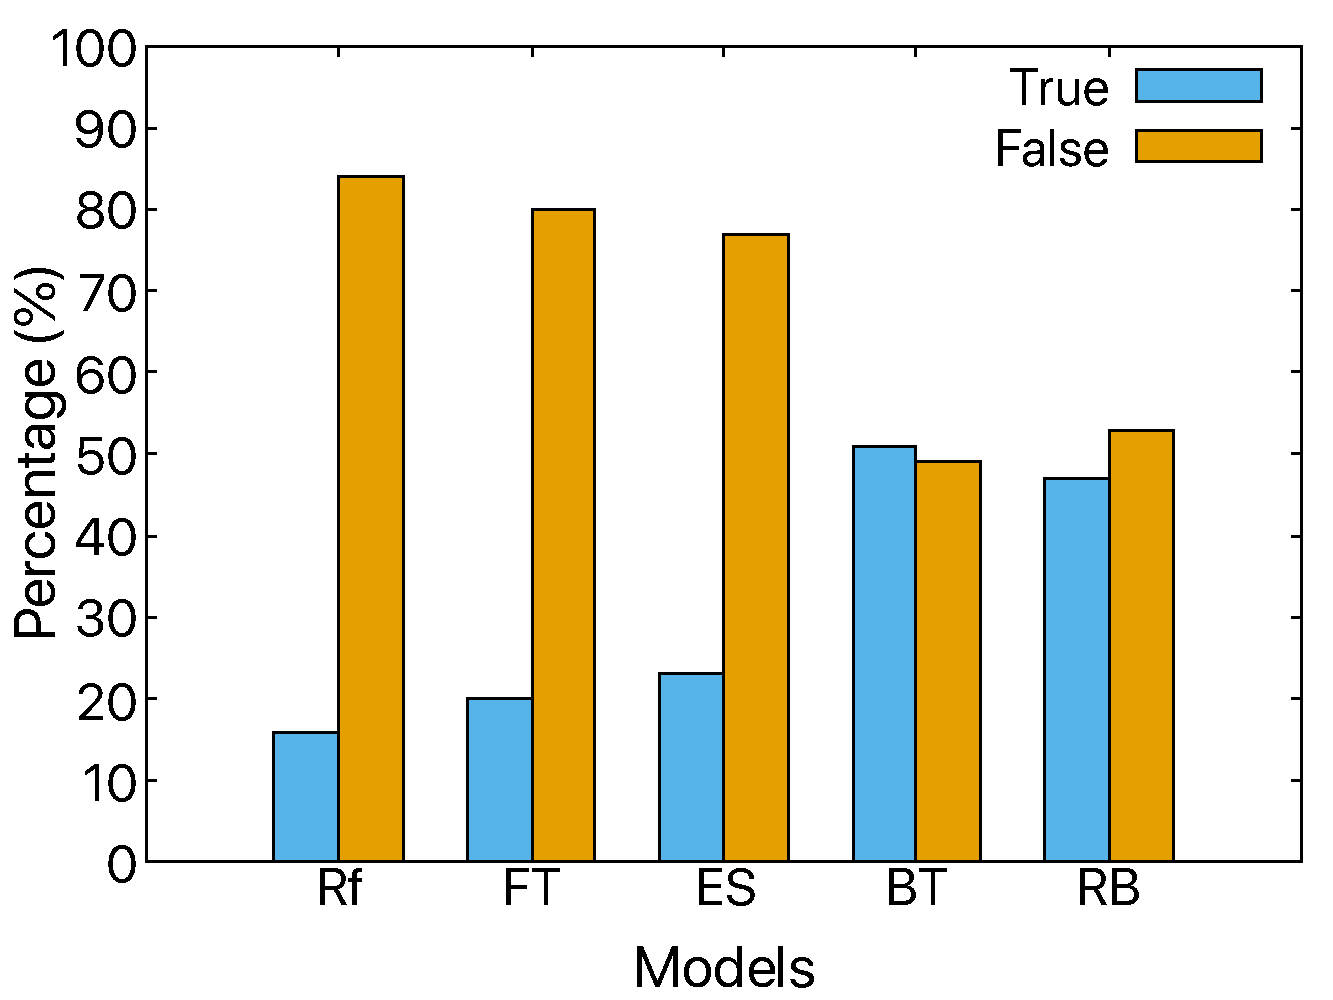
\includegraphics[width=\columnwidth]{figures/emnlp/threw-roc.pdf} 
    \caption*{ROC中的线索``threw''}
    \label{fig4:cue_threw}
    \end{minipage}
    \caption{四个不同模型的分布测试示例。}
    \label{fig4:cue_result}
    \end{figure}

在\figref{fig4:cue_result}中,我们展示了三个引人关注的发现。这些
柱状图代表了四个模型基于每个预测标签的分布百分比。$R_f$表示具有特定特征的训
练数据分布。我们注意到,在MNLI数据集中的``no''线索上,所有模型在\tabref{tab4:bias}中均获
得了正$\Delta$值,尤其是FastText。与准确性测试一致,我们发现在有``no''线索的情况
下,FastText和ESIM的预测标签分布偏差在\figref{fig4:cue_result}中得到了加强。它们
更倾向于预测``矛盾''类别,甚至超过了训练数据中的基线。与此相比,BERT和RoBERTa的预
测分布更加适度地遵循了训练数据。

尽管``no''线索在影响模型方面表现出一定的有效性,但``above''这一线索却并不那
么成功。\figref{fig4:cue_result}显示,在ARCT数据集中,ESIM的预测结果
分布与训练数据完全相反,这解释了\tabref{tab4:bias}中的$\Delta$值为-8.43,并
暗示即使数据中存在线索,模型也可能不会利用它。同样,BERT和RoBERTa在``speaking''线索
上的低$\Delta$值也解释了它们在\tabref{tab4:bias}中的表现。

特别地,``threw''线索为BERT提供了一个例外情况,因为在分布测试中的结果与准确性测试不一致:
尽管BERT在准确性偏差上表现很高,但其预测分布却相对均匀。我们并没有遇到很多这样的矛
盾情况。然而,当这种情况确实发生时,如在这个例子中,我们认为BERT可能没有真正利用``threw''这一
线索。

通过上述分析,我们不仅揭示了数据集中的线索和特征,还展示了这些线索对不同模型性能的影响。这
些发现为深入理解模型行为提供了宝贵的洞见,并为未来的数据集设计和模型开发提供了重要的指导.

\subsubsection*{3. 案例研究}
\label{sec4:mitigatingbiases}
\begin{figure*}[th]
\centering
\includegraphics[width=0.9\columnwidth]{figures/emnlp/prompt.eps}
\caption{提示语(prompt)。}
\label{fig4:prompt}
\end{figure*}
最近,OpenAI发布的大型语言模型(LLM)ChatGPT在自然语言处理(NLP)领
域引起了极大关注。ChatGPT,属于GPT-x系列模型\footnote{目前x的值为3.5或4,在我们的实验中,使用的是基于GPT-3.5的版本)}之一,
采用了类似InstructGPT\cite{ouyang2022training}的训练方法,即通过强化学习从人类反馈中学习(RLHF)。

在本节中,我们关注的是ChatGPT在零样本情况下是否受到偏见特征的影响。
具体来说,我们选择了一个聚焦于MNLI数据集中``no''一词的案例研究。我们的
目标是评估不同提示语的有效性,并基于这一单一偏见特征选择最佳提示语,以减轻偏见。

\subsubsection*{数据集}
\label{sec3:chatgptdata}
我们从MNLI数据集中挑选了测试实例,专注于``no''一词对ChatGPT性能的影响。
原始测试集包括3240个矛盾实例(Contradiction)、3463个蕴涵实例(Entailment)和3129
个中立实例(Neutral)。
含有``no''的实例分布为:矛盾229个,蕴涵38个,中立46个。

为了测试准确性,我们选取了所有含有``no''的313个实例,并从未包含``no''的测试集
中随机挑选了相同数量的实例,以确保评估的平衡性。

在分布测试中,我们从每种分类标签中各选取了38个含``no''的实例,共计114个。

\subsubsection*{提示语}
如图\ref{fig4:prompt}所示,我们设计了四种提示语。第一种由 ChatGPT 自行生成,
我们询问它关于 MNLI 任务的最佳提示语是什么,并得到了Prompt 1。
第二种提示语受到先前工作~\cite{qin2023chatgpt}的启发。
第三和第四种提示语在前两种提示语的基础上加入了``Let’s think step by step''\cite{kojima2022large}的元素,
采用了``思维链''(Chain of Thought, CoT)的方法,这种修改方式在
提高 InstructGPT 在推理任务上的性能方面已被证明有效,如 Ouyang 等人在 2022 年的研究\cite{ouyang2022training}所示。


\subsubsection*{ICQ结果}
\label{sec3:chatgptacc}

\begin{table}[th]
\centering
\scriptsize
\begin{tabular}{c|ccc}
\toprule
\textbf{提示语} & 准确率(含``no'') & 准确率(不含``no'') & $\Delta Acc$ \\ \midrule
P1  & 74.34& 77.32& -2.98   \\ \hline
P2&  75.42& 74.18 & 1.24 \\ \hline
P1 + CoT  & 78.35& 77.28&1.07  \\ \hline
P2 + CoT&  76.67& 76.40&  0.27 \\ \hline
 \bottomrule
\end{tabular}
\caption{准确性测试结果(\%)。P1=提示语1,P2=提示语2。}
\label{tab4:accuracy}
\end{table}

\begin{figure}[th]
\centering
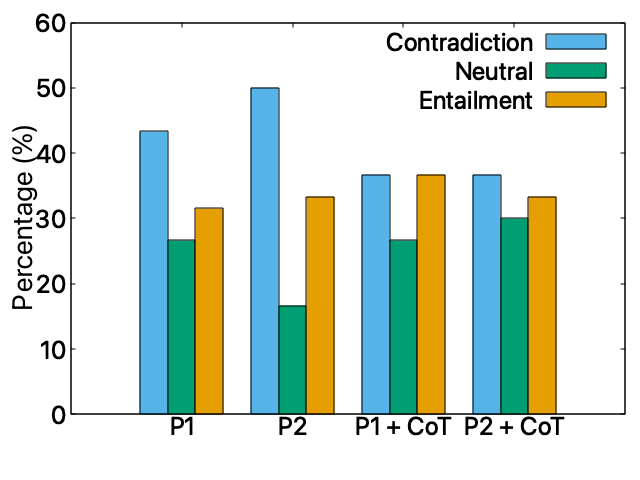
\includegraphics[width=0.6\columnwidth]{figures/emnlp/data/cue.png}
\caption{分布测试结果。}
\label{fig4:cue_chatgpt}
\end{figure}



我们使用不同的提示语对含有和不含有``no''的实例评估了模型的准确率。结果显示在\tabref{tab4:accuracy}中。
P1展示了负$\Delta$准确率,表明在存在``no''时难以泛化。
P2显示了正$\Delta$准确率,表明更好的泛化能力。
将``CoT''添加到两个提示语中都减少了偏见风险。
P1 + CoT在准确率(含``no'')方面显示了最显著的提升,但P2 + CoT有最小的绝对
$\Delta$准确率,表明对``no''的敏感性最低,是测试提示语中偏见风险最低的。

此外,我们分析了模型在不同提示语的压力测试集上的预测分布,如\figref{fig4:cue_chatgpt},该测试集包含了具有平衡标签分布的``no''一词。
分布测试结果揭示了P1和P2预测分布的不平衡,P1和P2倾向于预测矛盾。
添加``CoT''减轻了这些不平衡,导致更平衡的分布。
P2 + CoT在标签中呈现了最平衡的分布,支持其最低的偏见风险。

总之,我们的案例研究,特别是当关注``no''特征时,表明零样本ChatGPT可以受到偏见特征的影响。提示语的选择显著影响其性能。在评估``no''特征时,P2 + CoT在两项测试中显示了最低的偏见风险。``CoT''策略在减少这一特定特征的偏见风险方面似乎是有效的。然而,重要的是要注意,我们的发现,特别是关于``no''特征,表明ChatGPT推荐的自我提示语(P1)可能并不总是最优的。这强调了人类干预和持续探索的重要性,以优化性能并最小化偏见风险。未来的研究和结论将受益于更细致和针对特定特征的分析。

        

\subsection{本章小结}

在本章节的小结中,我们深入剖析了常识性推理模型鲁棒性不足的核心问题,并探讨了这一现象背后的深层原因。我们着重分析了模型在学习过程中缺乏人类的稳固推理能力,探求了模型究竟学习到了什么。为了深入理解这一问题,我们引入了两种创新的测试框架,目的是对相关问题进行更精细的分析与理解。

鉴于模型性能与数据密切相关,我们从宏观和微观两个角度出发,对数据中的偏见线索及模型的偏见进行了全面的评估和分析。在宏观层面,我们开发的测试框架通过对不同数据集上基于统计特征的简单分类模型的最高准确率进行评估,以及通过与多数选择(Majority)的偏差值来评估数据集中存在的偏差特征程度。我们将测试数据划分为简单(easy)和困难(hard)两类,以量化评估模型在识别和处理虚假特征方面的能力。这一方法揭示了模型对某些统计规律的过度依赖,有助于我们深入理解模型泛化能力的限制。

在微观层面,我们设计了ICQ(``I-see-cue'')框架。我们首先通过结合特征的分布不平衡性和训练集与测试集分布的相似性来定义``cueness score'',从而发现可能影响模型的关键特征,并评估数据集中存在的问题。ICQ通过多维特征划分和细致的性能分析,探究模型在不同特征上的准确性和分布表现。此外,我们还开发了一种直观的可视化工具,以更有效地识别和理解模型性能差异的根源。

值得一提的是,在微观分析中,我们还对ChatGPT进行了案例分析,证明了ICQ框架的广泛适用性,能够为多种模型提供深入的分析。

总体而言,本研究的主要贡献在于这两种高度创新的分析框架,它们为深入理解和提升常识性推理模型的鲁棒性开辟了新途径。通过结合宏观与微观方法,我们能够全面评估模型在处理复杂数据时的行为模式,特别是在识别潜在虚假特征方面的能力。这些成果不仅揭示了模型的潜在薄弱环节,也为未来设计更健壮、更可解释的人工智能系统奠定了一定的基础。
%iconip conclusion
%我们解决了自然语言理解和推理数据集中存在的统计偏差这一关键问题。我们提出了一个轻量级框架,
%自动识别多项选择自然语言理解(NLU)相关数据集中的潜在偏差,并评估为这些数据集设计的模型的健壮性。
%我们的实验结果证明了这一框架在检测数据集偏差和评估模型性能方面的有效性。此外,我们的方法在过滤有偏见的训练数据方面展现了潜力,
%从而促进了具有更强推理能力的模型的发展。

%作为未来的工作,我们计划进一步调查NLU数据集中偏差的本质,并探索更复杂的技术来检测和减轻这些偏差。
%此外,我们打算将我们的框架扩展到多项选择设置之外的其他类型的NLU任务。通过持续改进我们对数据集偏差及其对模型性能影响的理解,
%我们希望为开发更健壮、准确且可靠的NLU模型做出贡献,这些模型能够更好地泛化到现实世界应用中。

%我们的轻量级框架ICQ能够识别多项选择NLU数据集中的偏见和线索,从统计角度阐明模型行为。在多样化任务上的广泛实验验证了ICQ揭示数据集和模型偏见的效率。通过对ChatGPT的案例研究,我们探索了其线索,提供了实际指导。ICQ促进了我们对大型语言模型的理解和优化,推动了健壮、无偏见的人工智能系统的创建。

\newpage
\null
\newpage